\begin{frame}{Méthode de complétion}
  \begin{center}
    \begin{tikzpicture}
      \onslide<5->
      \draw[fill=fig-color-ri] (4,0) ellipse (5 and 2.2);
      \node (r*i) at (7.75,0) {$Prog'$};

      \onslide<4->
      \draw[fill=fig-color4] (3,0) ellipse (4 and 1.9);
      \node (...) at (5.75,0) {$\cdots$};
      
      \onslide<3->
      \draw[fill=fig-color3] (2,0) ellipse (3 and 1.6);
      \node (r2i) at (4,0) {$R^2(Prog)$};

      \onslide<2->      
      \draw[fill=fig-color2] (1,0) ellipse (2 and 1.3);
      \node (ri) at (1.75,0) {$R(Prog)$};

      \onslide<1->
      \draw[fill=fig-color-i] (0,0) ellipse (1 and 1);
      \node (i) at (0,0) {$Prog$};
    \end{tikzpicture}
  \end{center}
\end{frame}

\begin{frame}{\csclause}
  \begin{itemize}[<+->]
  \item Prédicats avec un nombre fixe d'arguments
  \item Propriétés des conjonctions d'atomes $B = A_1, ..., A_n$
    \begin{itemize}
    \item plat : $\forall A_i \in B, \forall t_j \in P(t_1, ..., t_n) = A_i, t_j$ est une variable
    \item linéaire : chaque variable dans $B$ n'apparaît qu'une seule fois
    \item $\emptyset$ : conjonction d'atomes vide : plat et linéaire
    \end{itemize}
    \vspace{\baselineskip}
  \item \csclause : $H \leftarrow B$ avec $B$ plat et linéaire \\~

  \item $P(f(g(x,y)),a) \leftarrow Q(x,y)$ : \csclause
  \item $P(x) \leftarrow Q(x),Q_2(g(x))$ : Pas une \csclause
  \end{itemize}
  
\end{frame}

\begin{frame}{\csprogramme}
  \begin{itemize}[<+->]
  \item \csprogramme : Ensemble de \csclauses
  \item Opérateurs
    \begin{itemize}
    \item $G \leadsto G'$ : (résolution prolog) \\
      $\exists H \leftarrow B \in Prog$ et $\exists \sigma$ \\
      t.q. $A \in G$ avec $\sigma(A) = \sigma(H)$ (unification)\\
      et $G' = \sigma(G)$ avec $\sigma(A)$ remplacé par $\sigma(B)$
    \item $G \rightarrow G'$ : (résolution faible) \\
      Comme ci-dessus mais avec $A = \sigma(H)$ (filtrage)
    \end{itemize}
  \end{itemize}
  \onslide<5>
  \begin{block}{Langage d'un \csprogramme}
    Soit $\vec{t}$ des termes clos.
    $\vec{t} \in \mathcal{L}_{Prog}(P)$ si et seulement si $P(\vec{t}) \leadsto^*_{Prog} \emptyset$.
  \end{block}
\end{frame}

\begin{frame}{Exemple}
  \begin{itemize}[<+->]
  \item $Prog$ =
    \begin{itemize}
    \item \color<6>{focusColor}$P(f(x,y)) \stackrel{1}{\leftarrow} Q(x, y)$ \\
    \item \color<7>{focusColor}$Q(v(x), w(y)) \stackrel{2}{\leftarrow} Q(x, y)$ \\
    \item \color<8>{focusColor}$Q(a, a) \stackrel{3}{\leftarrow} $
    \end{itemize}
  \item $f(v(a),w(a)) \in \mathcal{L}_{Prog}(P)$ ?
    \begin{itemize}
    \item $P(f(v(a),w(a))) \leadsto Q(v(a), w(a))$ \\
    \item $Q(v(a), w(a)) \leadsto Q(a, a)$ \\
    \item $Q(a, a) \leadsto \emptyset$
    \item Oui, $f(v(a),w(a)) \in \mathcal{L}_{Prog}(P)$
    \end{itemize}
  \item $\mathcal{L}_{Prog}(P) = \{f(v^n(a),w^n(a)) | n \in \mathbb{N}\}$
  \end{itemize}
\end{frame}

\begin{frame}{L'algorithme de complétion}
  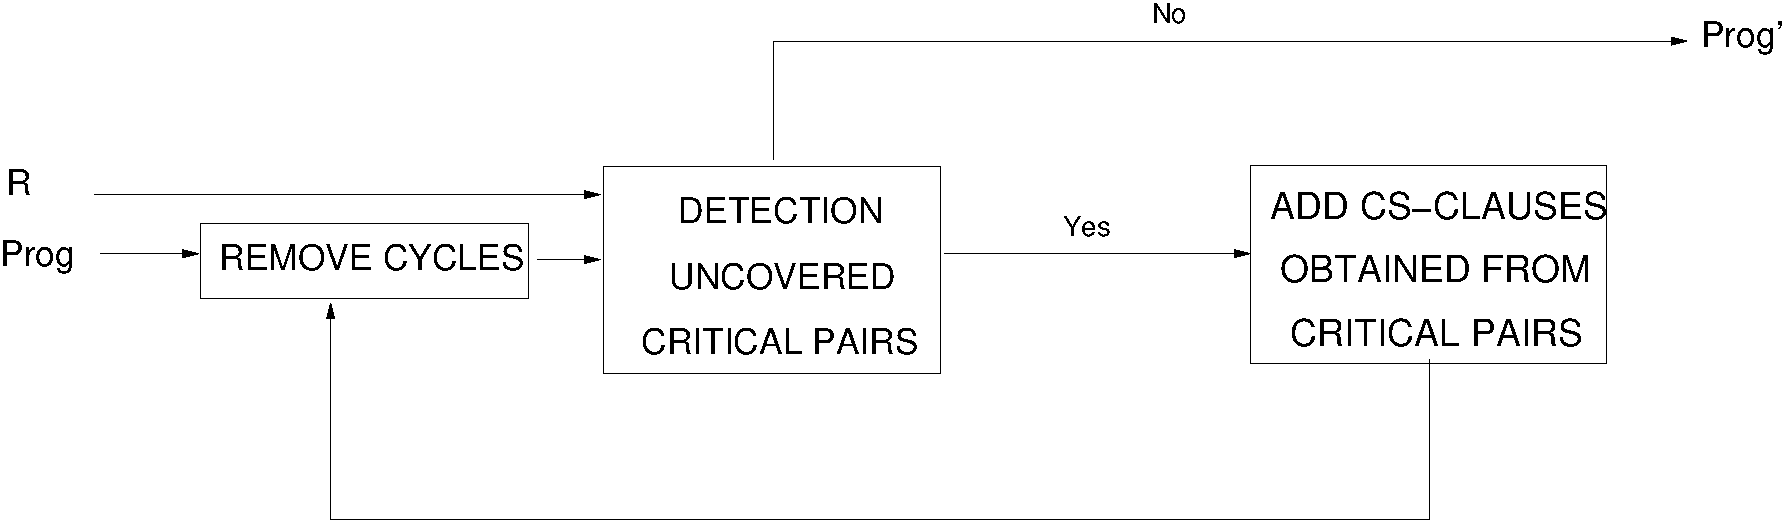
\includegraphics[width=\linewidth]{media/schema.pdf}\\
  \begin{itemize}[<+->]
  \item Le \csprogramme initial est
    \begin{itemize}
      \item non copiant
      \item normalisé
    \end{itemize}
    \vspace{\baselineskip}
  \item Le système de réécriture est
    \begin{itemize}
      \item linéaire
    \end{itemize}
  \end{itemize}
\end{frame}

\begin{frame}{Paires critiques}
  \begin{itemize}[<+->]
  \item ${\color<3>{focusColor}l} \rightarrow r \in R$
  \item $P(..., {\color<3>{focusColor}t_i}, ...) \leftarrow B \in Prog$
  \end{itemize}
  \begin{overprint}
    \onslide<3>
    $P(..., l, ...)$
    \onslide<4>
    $P(..., l, ...) $ \hfill $ \xrsquigarrow{~~~~~~~~~~~~~~~~~~~~~~~~~}^+_{[\sigma]} $ \hfill $ G$ avec $G$ plat \\
    \onslide<5>
    $P(..., l, ...) $ \hfill $ \xrsquigarrow{~~~~~~~~~~~~~~~~~~~~~~~~~}^+_{[\sigma]} $ \hfill $ G$ avec $G$ plat \\
    \begin{center}
      
\includegraphics[width=.8\linewidth]{media/CP1.pdf} \\
    \end{center}
    \onslide<6>
    $P(..., l, ...) $ \hfill $ \xrsquigarrow{~~~~~~~~~~~~~~~~~~~~~~~~~}^+_{[\sigma]} $ \hfill $ G$ avec $G$ plat \\
    \begin{center}
      
\includegraphics[width=.8\linewidth]{media/CP2.pdf} \\
    \end{center}
  \end{overprint}
  \onslide<5->
  $\sigma(P(..., r, ...)) \leftarrow G$ : paire critique
\end{frame}

\begin{frame}{Exemple}
  \begin{itemize}[<+->]
  \item $R$ : $\{{\color<3>{focusColor}g(h(y))} \rightarrow f(y) \}$
  \item $Prog$ : $\{{\color<4>{focusColor}{\color<3>{focusColor}P(g(x))} \leftarrow Q(x)}; {\color<5>{focusColor}Q(h(x)) \leftarrow Q'(x)}; Q'(a) \leftarrow \}$
  \end{itemize}
  \begin{overprint}
    \onslide<3>
    $P(g(h(y)))$
    \onslide<4>
    $P(g(h(y))) \xrsquigarrow{~~~~~~~~~~~~~~~~~~~~~~~~~} Q(h(y)) $
    \onslide<5>
    $P(g(h(y))) \xrsquigarrow{~~~~~~~~~~~~~~~~~~~~~~~~~} Q(h(y)) \xrsquigarrow{~~~~~~~~~~~~~~~~~~~~~~~~~} Q'(y)$ \\
    \onslide<6>
    $P(g(h(y)))$ \hfill $ \xrsquigarrow{~~~~~~~~~~~~~~~~~~~~~~~~~}^+_{[\sigma]} $ \hfill $ Q'(y)$ et $Q'(y)$ plat \\
    \onslide<7>
    $P(g(h(y)))$ \hfill $ \xrsquigarrow{~~~~~~~~~~~~~~~~~~~~~~~~~}^+_{[\sigma]} $ \hfill $ Q'(y)$ et $Q'(y)$ plat \\
    \begin{center}
      
\includegraphics[width=.8\linewidth]{media/CP1.pdf} \\
    \end{center}
    \onslide<8>
    $P(g(h(y)))$ \hfill $ \xrsquigarrow{~~~~~~~~~~~~~~~~~~~~~~~~~}^+_{[\sigma]} $ \hfill $ Q'(y)$ et $Q'(y)$ plat \\
    \begin{center}
      
\includegraphics[width=.8\linewidth]{media/CP2.pdf} \\
    \end{center}
  \end{overprint}
  \onslide<7->
  $\sigma(P(f(y))) \leftarrow Q'(y)$ : paire critique
\end{frame}

\begin{frame}{Le problème}
  \begin{itemize}[<+->]
  \item $Prog = \{ P(f(x,x)) \leftarrow Q(x).\,
    Q(a) \leftarrow .\,
    Q(b) \leftarrow .\}$
  \item $R = \{a \rightarrow b\}$ \\~

  \item Une paire critique : $Q(b) \leftarrow$
  \item Elle est convergente \\~

  \item $f(a, a) \in \mathcal{L}_{Prog}(P)$
  \item $f(a, a) \rightarrow_R f(b, a)$
  \item mais $f(b, a)$ et $f(a,b) \notin \mathcal{L}_{Prog}(P)$
  
  \end{itemize}
\end{frame}
